\documentclass[11pt,twoside]{report}


%\newif\ifmynotes
%\mynotesfalse
%\mynotestrue

\usepackage{ece586}

\newcommand{\vecnot}[1]{#1}

%% TOGGLE  Notes
%\newif\ifgnotes
%\anstrue

%\ifmynotes
%	\definecolor{note_text}{rgb}{1,1,1}		
%	\newcommand{\gskip}{\vspace*{1cm}}
%	\newcommand\gnote[1]{\protect\leavevmode\begingroup\Huge\color{note_text}#1\endgroup\ignorespaces}
%	\newenvironment{gnotes}{\Huge\color{red}}{\ignorespacesafterend}
%\else
%	%\newcommand{\gnote}[1]{#1\ignorespaces} 	% make commands do nothing. 
%	\definecolor{note_text}{rgb}{0,0,.7}
%	\newcommand\gnote[1]{\protect\leavevmode\begingroup\color{note_text}#1\endgroup\ignorespaces}
%	\newenvironment{gnotes}{\color{red}}{\ignorespacesafterend}
%%	\newcommand{\gskip}{}
%\fi
%


\begin{document}

\lectureheader{0}{Introduction}





\section{Overview} 

\begin{itemize}
\item The is an applied math class for graduate studeinds in data science and signal processing. The high level goals are: 
\begin{itemize}
  \item Review and extend undergraduate knowledge  of  linear systems, vector spaces, matrices, and optimization
  
  \item  Teach the vocabulary and basic mathematical concepts necessary to read and understand papers and textbooks
  
  \item Emphasis is on general techniques that extend to advanced problems
   


\end{itemize}

\item Topics and applications




\begin{itemize}
  \item Logic and set theory
  \item Metric spaces and topology\\  $\implies $ analysis of iterative algorithms

  \item Linear algebra: Normed and inner-product spaces\\
  $\implies $  spaces of functions and Markov chains
  \item Approximation and projection\\
   $\implies $   function approximation and machine learning    
  \item The four fundamental subspaces and singular value decomposition\\
   $\implies $  dimensionality reduction
  \item Optimization in Vector Spaces
  $\implies $  duality bounds in convex optimization
\end{itemize}


\end{itemize}

\section{Example Problems}


\subsection{Solving a linear system of equations} 


\begin{itemize}
  \item Suppose you know a vector $\vecnot{b}$ satisfies \[A \vecnot{x} = \vecnot{b}\] for an invertible matrix $A$. 
  \begin{itemize}
 \item  To compute $\vecnot{x}$, you could multiply by $A^{-1}$ to get 
  \[A^{-1} \vecnot{b} = A^{-1} (A \vecnot{x}) = \vecnot{x}\!\!\!\!\!\!\!\!\!\]
  
  \item But, what if \textcolor{blue}{$A$ is not known perfectly}?
  
  \item  Let's assume we know $\hat{A} = A + E$ where the \textcolor{blue}{error matrix $E$ is ``small''}
  
  \item  Now, we can compute $\hat{\vecnot{x}} = \hat{A}^{-1} \vecnot{b}$. \textcolor{blue}{But, what can we say about $\vecnot{x}-\hat{\vecnot{x}}\;$?} \vspace{3mm}

\end{itemize}

\item  The mathematical study of ``closeness'' is called \textbf{topology} 

\begin{itemize}
  \item Define ``distance''  between objects (e.g., vectors, matrices)
  \item Define a constant $c(\hat{A})$ such that
  \[ \text{distance}(\vecnot{x},\hat{\vecnot{x}}) \leq c(\hat{A}) \; \text{distance}(A,\hat{A}) = c(\hat{A}) \; \text{length}(E)  \]
\end{itemize}
\end{itemize}


\subsection{Approximation by simple functions} 
\begin{itemize}

  \item  Suppose you want to find a 3rd-order polynomial that gives a \textcolor{blue}{``good'' approximation} of a function \textcolor{blue}{$f(x)$} on the interval $[0,1]$.
  
  
  \begin{itemize}
  
  \item A key question is, ``What do we mean by good?'' max error? avg error?
  
  \item A standard approach is to minimize the \textcolor{blue}{mean squared error} and this gives
  \[ \min_{a_0,a_1,a_2,a_3} \int_0^1 \left[ f(x) - (a_0+a_1 x+ a_2 x^2+a_3 x^3) \right]^2 dx \]
  
  \item  Given $f(x)$ and the ability to integrate, one \textcolor{blue}{can solve this via brute force}
  
  \item  This course will show there is also an \textcolor{blue}{simple intuitive approach}


\end{itemize}

\item  Solution via orthogonality and linear algebra 

\begin{itemize}

  \item  Compute $a_0,a_1,a_2,a_3$ using system of 4 \textbf{linear equations}  ($k=0,1,2,3$) given by
  \[ \int_0^1 (a_0+a_1 x+ a_2 x^2+a_3 x^3) x^k dx = \int_0^1 f(x)x^k dx. \]

 \end{itemize}
 \begin{center}
 % \begin{tikzpicture}[overlay,remember picture,shift={(11.8,1.05)}]
    \begin{tikzpicture}%[overlay,remember picture,shift={(11.8,1.05)}]
  \begin{axis}[small,width=4in,height=2in,xmin=0,xmax=1,ymin=0,ymax=1,grid=both]
   \addplot[blue,domain=0:1,thick,samples=100,-] { (0.5+0.4*(1-x)*cos(deg(8*x)))^2 };
    \addplot[red,domain=0:1,dashed,samples=100] { (0.5+0.4*(1-x)*cos(deg(8*x)))^2 - 0.1};
  \addplot[red,domain=0:1,dashed,samples=100] { (0.5+0.4*(1-x)*cos(deg(8*x)))^2 + 0.1};
\addplot[green!50!black,domain=0:1,thick,samples=200] { 0.957379 - 5.55126 * x + 10.9672 * x^2 - 6.21221 * x^3 };
  \end{axis}
\end{tikzpicture}
\end{center}
  \end{itemize}
 


\subsection{Optimization of a convex function} 

\begin{itemize}

\item Let $f(x)$ be a function on the the real interval $[a,b]$
\begin{itemize}
\item A \textbf{chord} of $f$ is a linear connecting $(x, f(x))$ and $(y, f(y))$. 
\item function $f$ is convex $\iff $ all chords lie above the function, i.e., for all $\lambda \in [0,1]$, 
\[ f(\lambda x +(1-\lambda) y) \leq \lambda f(x) + (1-\lambda) f(y) \] 

\item Convexity implies all local minima have the same \textbf{minimum value} 


\end{itemize}

\begin{center}
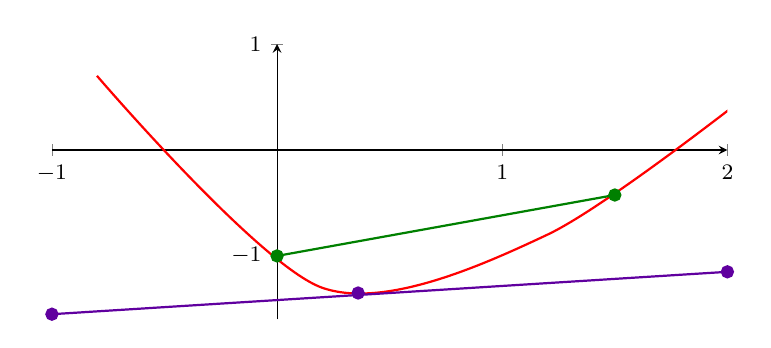
\begin{tikzpicture}%[overlay,remember picture,shift={(10.5,0.35)}]
  \begin{axis}[axis x line=center, axis y line=center, small,width=4in,height=2in,xmin=-1,xmax=2,ymin=-1.6,ymax=1,   xtick = {-1,1,2}]
\addplot[red,smooth,thick,-] coordinates  {(-0.8,0.7) (0.2,-1.3) (1.2,-0.8) (2.2,0.7)};
 \addplot[mark=*, thick, green!50!black] coordinates {(0,-1)(1.5,-0.425)};
 \addplot[mark=*, thick, purple!50!blue] coordinates {(0.36,-1.35)};
\addplot[mark=*, thick, purple!50!blue] coordinates {(-1,-1.55)(2,-1.15)};
  \end{axis}
\end{tikzpicture}
\end{center}

\item \textbf{Question:} Can we compute a simple lower bound on the minimum value? 


\begin{itemize}

\item Solution via \textbf{tangent line} 
\item A convex function lies above any tangent line and 
  \[ \min_{x\in [a,b]} f(x) \geq \min_{x\in [a,b]} \left[ f(x_0)+(x-x_0) f'(x_0) \right] 
  \]
  
  \item The minimum of the tangent provides a lower bound for any choice of $x_0$. 
    \item Maximizing over $x_0$ recovers the minimum!
\end{itemize}
\end{itemize}



\bibliographystyle{alpha}%{IEEEtran}
\bibliography{/Users/galenreeves/Dropbox/Library/long_names,/Users/galenreeves/Dropbox/Library/library} 
\end{document}

